\documentclass[aspectratio=169,t,10pt,table]{beamer}
\usepackage{slides}
\usepackage{makecell}
\usepackage{booktabs}
\usepackage{ulem}
\usepackage{amsmath,amssymb,mathrsfs}
\usepackage{tabularray}        
\usepackage{multirow}
\usepackage{rotating}
\usepackage{tikz}
\definecolor{accent2}{HTML}{942300}
\definecolor{accent}{HTML}{006896}

\newcommand{\vs}{\vspace{0.1in}}
\newcommand{\vbs}{\vspace{0.2in}}

\newtheorem{assumption}{Assumption}
\newtheorem{proposition}{Proposition}

\newcommand{\indicator}[1]{\mathbbm{1}_{\left\{ {#1} \right\} }}

\newenvironment{fignote2}[1]
{
\par
\smallskip
\begin{minipage}{#1}
\tiny
}
{
\end{minipage}
}

%Set the 'itemize' bullets and linespacing
%\setlist[itemize,1]{label=$\blackdot$, itemsep=1.5ex}         %triangle for first level
%\setlist[itemize,2]{label=$\blacktriangleright$, itemsep=0.5ex}         %triangle for second level
%\setlist[enumerate,1]{label=\arabic*.,font=\bfseries, itemsep=1.5ex}    %for numbered lists, bold the numbers


%%%%%%%%%%%%%%%%%%%%%%%%%%%%%%%%%%%%%%%%%%%%%%%%%%%%%%%%%%%%%%%%%%%%%%%%%%%
\title{\textbf{Tariffs, Manufacturing Employment, and Supply Chains}}
\author{\text{Joseph B. Steinberg}\ |\ \text{University of Toronto \& NBER}\vspace{4pt}}
\date{Tariffs and Trade Policy: Past, Present, and Future\ |\  NC State |\ December 2025}
\addbibresource{bib.bib}

%%%%%%%%%%%%%%%%%%%%%%%%%%%%%%%%%%%%%%%%%%%%%%%%%%%%%%%%%%%%%%%%%%%%%%%%%%%
\begin{document}


%%%%%%%%%%%%%%%%%%%%%%%%%%%%%%%%%%%%%%%%%%%%%%%%%%%%%%%%%%%%%%%%%%%%%%%%%%%
\begin{frame}[noframenumbering,plain]
\maketitle
\end{frame}

%%%%%%%%%%%%%%%%%%%%%%%%%%%%%%%%%%%%%%%%%%%%%%%%%%%%%%%%%%%%%%%%%%%%%%%%%%%
\begin{frame}[plain]
\centering
\vspace{0.75cm}
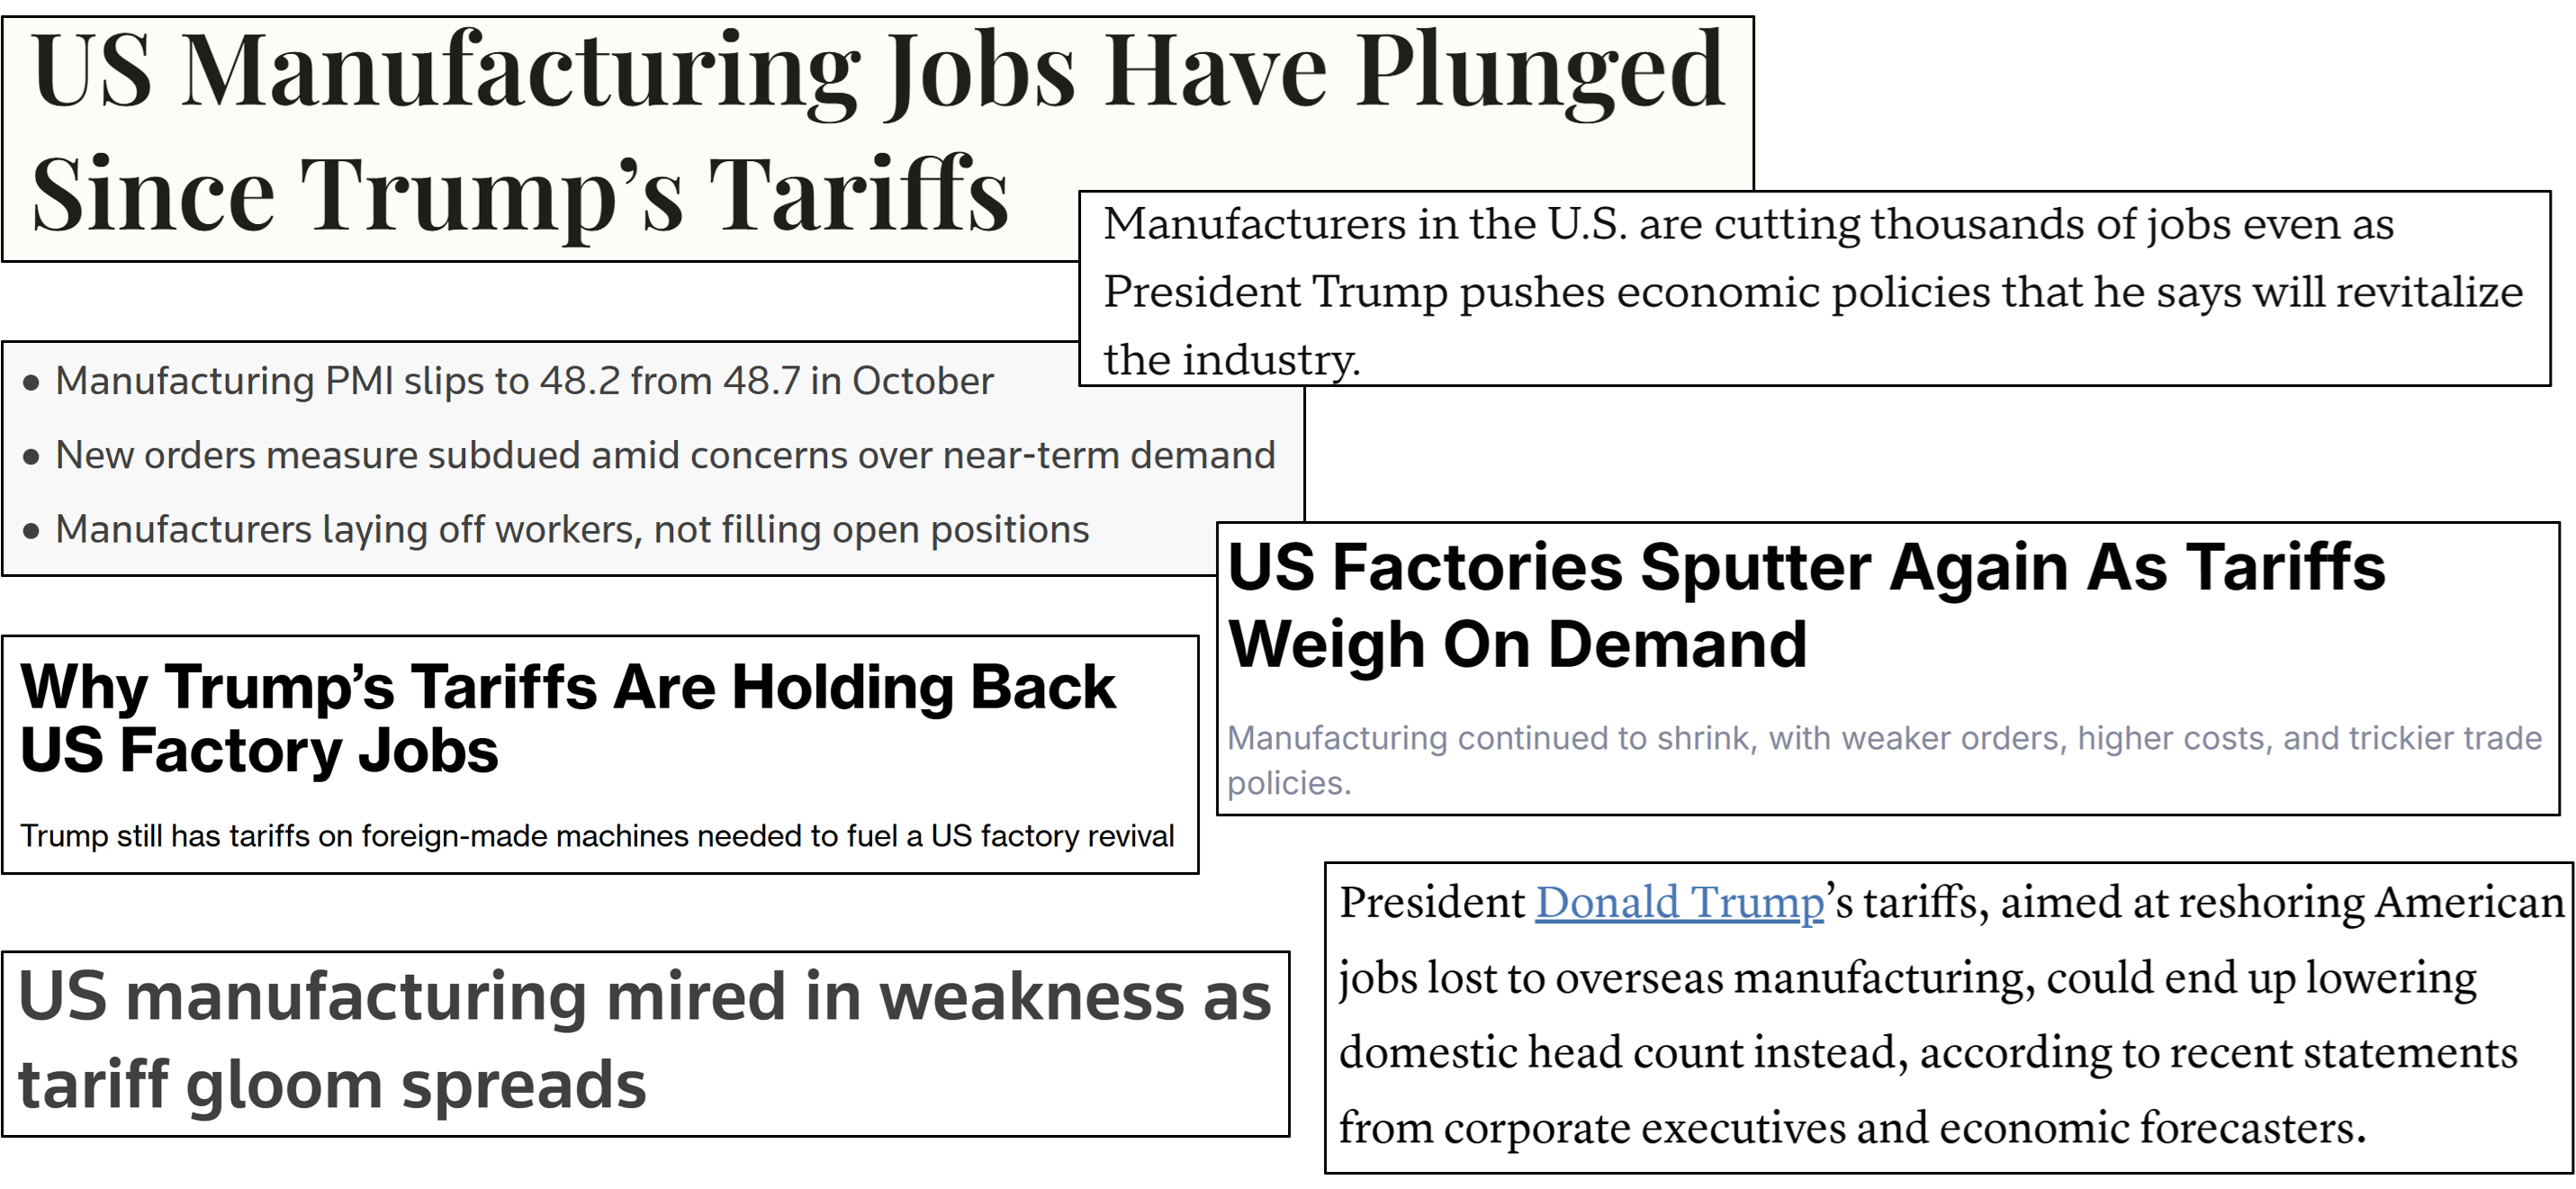
\includegraphics[width=\textwidth]{tariff_news.png}
\end{frame}


%%%%%%%%%%%%%%%%%%%%%%%%%%%%%%%%%%%%%%%%%%%%%%%%%%%%%%%%%%%%%%%%%%%%%%%%%%%
\begin{frame}[noframenumbering,plain,t]{Motivation}

\begin{itemize}\addtolength{\itemsep}{1ex}
    \item Stated goal of Trump tariffs: ``reindustrialize'' U.S. economy
    \begin{itemize}\addtolength{\itemsep}{0.5ex}
        \item Can it work?
        \item Best way to do it?
        \item How long will it take?
    \end{itemize}
    \item Problem 1: Tariffs raise costs for downstream industries
\begin{itemize}\addtolength{\itemsep}{0.5ex}
        \item Steel tariffs during 1st Trump admin increased steel employment but\ldots
        \item Destroyed $\sim$10x more jobs in other mfg sectors (Cox and Russ, 2020; Flaaen and Pierce 2024)
        \item Reduced export growth in other mfg sectors (Handley et al. 2020)
    \end{itemize}
\item Problem 2: Frictions slow adjustment \& cause short-term pain
\begin{itemize}\addtolength{\itemsep}{0.5ex}
\item Factors: Need to build new factories, get workers to switch occupations
    \item Supply chains: Transitory shocks in upstream sectors cause persistent disruptions in downstream sectors (Tsyvinski and Liu 2024)
\end{itemize}
\item This paper: short vs. long-run effects of tariffs on mfg employment in general equilibrium
\end{itemize}

\end{frame}

%%%%%%%%%%%%%%%%%%%%%%%%%%%%%%%%%%%%%%%%%%%%%%%%%%%%%%%%%%%%%%%%%%%%%%%%%%%
\begin{frame}[noframenumbering,plain,t]{What I do}

\begin{itemize}\addtolength{\itemsep}{1ex}
    \item Build multi-sector, multi-country dynamic GE model of US economy
    \begin{itemize}\addtolength{\itemsep}{0.5ex}
        \item Starting point: Kehoe et al. (2018)
        \item Manufacturing split into 4 subsectors that differ by trade elasticity and upstreamness:
        \begin{itemize}\addtolength{\itemsep}{0.3ex}
            \item ``Oil:'' upstream, high elasticity
            \item ``Steel:'' upstream, low elasticity
            \item ``Toys:'' downstream, high elasticity
            \item ``Cars:'' downstream, low elasticity
        \end{itemize}
        \item Supply-chain adjustment frictions as in Tsyvinski and Liu (2024)
    \end{itemize}
   \item Simulate effects of tariffs on sectoral employment dynamics
   \begin{itemize}
       \item Target specific sectors vs. across the board
        \item Baseline vs. frictionless model
       \item Target one country vs. entire world
       \item Passive trade partners vs. retaliation
   \end{itemize}
\end{itemize}

\end{frame}

%%%%%%%%%%%%%%%%%%%%%%%%%%%%%%%%%%%%%%%%%%%%%%%%%%%%%%%%%%%%%%%%%%%%%%%%%%%
\begin{frame}[noframenumbering,plain,t]{What I find}

\begin{itemize}\addtolength{\itemsep}{1ex}
    \item Tariffs can raise overall manufacturing employment
    \begin{itemize}
    \item Tariff on all mfg sectors: 1.75pct increase
        \item Best case: tariff on ``toys'' only, 3pct increase
        \item Worst case: tariff on ``cars'' only, 2pct decrease
    \end{itemize}
    \item Net effect on overall mfg employment masks significant reallocation between mfg sectors
    \begin{itemize}
       \item Tariff on all mfg sectors: only ``toys'' grows, all other sectors shrink
        \item ``Cars'' tariff: employment in ``cars'' rises slightly, other 3 mfg sectors all shrink at least 2x more
    \end{itemize}
    \item Employment may fall in short run before eventually rising
    \begin{itemize}
        \item Tariff on all mfg sectors: employment rises by 1.75pct in long run, but falls by 1.25pct in short run and remains depressed for 11 years
    \end{itemize}
    \item If other countries retaliate, long-run gains disappear and short-run losses double
\end{itemize}

\end{frame}

%%%%%%%%%%%%%%%%%%%%%%%%%%%%%%%%%%%%%%%%%%%%%%%%%%%%%%%%%%%%%%%%%%%%%%%%%%%
\begin{frame}[noframenumbering,plain,t]{Related literature}

\begin{itemize}\addtolength{\itemsep}{1ex}
\item Trade war economics:  {\small{Steinberg (2020), Carroll and Hur (2023), Flaeen and Pierce (2024), Alessandria et al. (2025ab), Bianchi and Coulibaly (2025), Cavallo et al. (2025), Cuba-Borda et al. (2025), Ignatenko et al. (2025), Itskhoki and Mukhin (2025), Pujolas and Rossback (2025)}}
\begin{itemize}
    \item This paper: short-run vs. long-run effects on manufacturing employment
\end{itemize}
    \item Structural change in open economies: {\small{Uy et al. (2013), Kehoe et al. (2018), Sposi (2019), Lewis et al. (2022), Sposi et al. (2025)}}
    \begin{itemize}
    \item This paper: tariffs as driving force; reallocation between manufacturing sub-sectors
\end{itemize}
    \item Global value chains:  {\small{Johnson and Noguera (2012), Antras et al. (2012), Caliendo and Parro (2014), Liu (2019), Liu and Tsyvinski (2024), Alessandria et al. 2023, Blanchard et al. (2024), Georgieva (2025)}}
       \begin{itemize}
    \item This paper: tariffs as a supply-chain disruption
\end{itemize}
\end{itemize}

\end{frame}



%%%%%%%%%%%%%%%%%%%%%%%%%%%
%%%%%%%%%%%%%%%%%%%%%%%%%%%
\begin{transitionframe}
Model
\end{transitionframe}

%%%%%%%%%%%%%%%%%%%%%%%%%
%%%%%%%%%%%%%%%%%%%%%%%%%
\begin{frame}[noframenumbering,plain,t]
  \frametitle{Overview}
  \begin{itemize}\addtolength{\itemsep}{1ex}
  \item Discrete time, perfect foresight 
  \item $I$ countries indexed by $i,j$ (subscripts)
  \item $S$ sectors indexed by $s,r$ (superscripts)
\item Agents:
    \begin{itemize}\addtolength{\itemsep}{0.5ex}
    \item Households: work, consume, invest, buy bonds
    \item Producers: $\text{gross output} = f(\text{labor}, \text{capital}, \text{intermediates})$
    \item Distributors: $\text{sector-specific Armington composite} = g(\text{domestic products},\text{foreign products})$
    \item Retailers: $\text{consumption} + \text{investment} = h(\text{sectoral composites})$
    \item Governments: levy import tariffs
    \end{itemize}
  \end{itemize}
\end{frame}

%%%%%%%%%%%%%%%%%%%%%%%%%
%%%%%%%%%%%%%%%%%%%%%%%%%
\begin{frame}[noframenumbering,plain,t]
  \frametitle{Producers}
  \begin{itemize}\addtolength{\itemsep}{1ex}
  \item Produce output using capital, labor, and intermediate inputs subject to labor adjustment costs
\begin{align*}
\small
   y^s_{i,t}=\left\{\lambda^{s,v}_i\left[(k^s_{i,t})^{\alpha^s_i} (\ell^s_{i,t})^{1-\alpha^s_i}\right]^{\frac{\eta-1}{\eta}}+\left[\sum_{r=1}^S \lambda^{s,r}_i (m^{s,r}_{i,t})^{\frac{\xi-1}{\xi}}\right]^{\frac{\eta-1}{\eta}\frac{\xi}{\xi-1}}\right\}^{\frac{\eta}{\eta-1}}-\phi_\ell \left(\frac{\ell^s_{i,t}}{\ell^s_{i,t-1}}-1\right)^2\ell^s_{i,t-1}
\end{align*}
\item Adjusting capital is also costly
\begin{align*}
     k^s_{i,t+1}=(1-\delta)k^s_{i,t}+\delta^{1-\phi_k}(x^s_{i,t})^{\phi_k} (k^s_{i,t})^{1-\phi_k}
\end{align*}
\item Choose $\{\ell^s_{i,t},k^s_{i,t},m^{s,1}_{i,t},\ldots,m^{s,S}_{i,t}\}_{t=0}^\infty$ to maximize PDV of dividends
\[\sum_{t=0}^\infty \Lambda_{i,t} \left[p^s_{i,t} y^s_{i,t}-w_{i,t}\ell^s_{i,t}-p^x_{i,t}x^s_{i,t}-\sum_{r=1}^S p^{m,r}_{i,t}m^{s,r}_{i,t}\right]\]
  \end{itemize}
\end{frame}

%%%%%%%%%%%%%%%%%%%%%%%%%
%%%%%%%%%%%%%%%%%%%%%%%%%
\begin{frame}[noframenumbering,plain,t]
  \frametitle{Distributors}
  \begin{itemize}\addtolength{\itemsep}{1ex}
  \item Combine domestic and foreign products into use-specific (final or intermediate) Armington composites subject to cost of substituting between suppliers
    \[q^{u,s}_{i,t}=\left[\sum_{j=1}^I \mu^{u,s}_{i,j}(z^{u,s}_{i,j,t})^{\frac{\zeta^{s}-1}{\zeta^{s}}}\right]^{\frac{\zeta^{s}}{\zeta^{s}-1}} - \sum_{j=1}^I\phi_u \left(\frac{z^{u,s}_{i,j,t}}{z^{u,s}_{i,j,t-1}}-1\right)^2 z^{u,s}_{i,j,t-1},\ u\in\{m,f\}\]
\vspace{-0.25cm}
    \begin{itemize}\addtolength{\itemsep}{0.5ex}
    \item Long-run trade elasticities, $\zeta^{s}$, vary by sector
    \item Adjustment frictions modeled as in Tsyvinski and Liu (2024)
    \item Lower short-run elasticities as in Krugman (1986)
    \end{itemize}
\item Choose $\{z^{u,s}_{i,1,t},\ldots,z^{u,s}_{i,I,t}\}_{t=0}^\infty$ to maximize PDV of dividends
\[\sum_{t=0}^\infty\Lambda_{i,t}\left[p^{u,s}_{i,t}q^{u,s}_{i,t}-\sum_{j=1}^I (1+\tau^s_{i,j,t}) z^{u,s}_{i,j,t}\right]\]
  \end{itemize}
\end{frame}

%%%%%%%%%%%%%%%%%%%%%%%%%
%%%%%%%%%%%%%%%%%%%%%%%%%
\begin{frame}[noframenumbering,plain,t]
  \frametitle{Retailers, households, and government}
  \begin{itemize}\addtolength{\itemsep}{1ex}
  \item Retailers: combine final-use sectoral composites into aggregate consumption and investment:
    \begin{align*}
      c_{i,t} = \left[\sum_{s=1}^S\varepsilon^{c,s}_{i} \left(z^{c,s}_{i,t}\right)^{\frac{\rho^c-1}{\rho_c}}\right]^{\frac{\rho_c}{\rho^c-1}},\quad x_{i,t} &= \left[\sum_{s=1}^S \varepsilon^{x,s}_{i} \left(z^{x,s}_{i,t}\right)^{\frac{\rho^x-1}{\rho_x}}\right]^{\frac{\rho_x}{\rho^x-1}}
    \end{align*}
  \item Households: work, consume, and save
  \begin{align*}
      \max_{\{c_{i,t},\ell_{i,t},b_{i,t+1}\}_{t=0}^\infty} \sum_{t=0}^\infty u_i(c_{i,t},\bar{\ell}_i-\ell_{i,t})\quad \text{s.t.}\quad p^{c}_{i,t} c_{i,t} + Q_t b_{i,t+1} = w_{i,t}\ell_{i,t} + \bar{p}_t b_{i,t} + \Pi_{i,t} + T_{i,t}
  \end{align*}
  \item Government:
  \begin{itemize}\addtolength{\itemsep}{0.5ex}
      \item Set tariffs $\tau^s_{i,j,t}$ on goods from country $j$'s sector $s$
      \item Today: Rebate tariff revenue lump-sum to households
      \item Future: Reduce other distortionary taxes or subsidize investment as in Alessandria et al. (2025)
  \end{itemize}
  \end{itemize}
\end{frame}

%%%%%%%%%%%%%%%%%%%%%%%%%
%%%%%%%%%%%%%%%%%%%%%%%%%
\begin{frame}[noframenumbering,plain,t]
  \frametitle{Equilibrium}
  \begin{itemize}\addtolength{\itemsep}{1ex}
    \item Sequence of prices and quantities that satisfy (i) household, retailer, distributor, and producer problems, and (ii) market clearing conditions
\item Steady-state equilibrium: if tariffs are constant, equilibrium converges in long run to situation where all p's and q's are constant
\item But no unique steady state! Continuum of steady states indexed by vector $b_{i,\infty}$ as in Kehoe et al. (2018) and Steinberg (2019, 2020)
\begin{itemize}\addtolength{\itemsep}{0.5ex}
\item Long-run trade imbalances are endogenous
\item Steady state determined by initial conditions and policy trajectory
\item Adjustment costs $\phi^m,\phi^f,\phi^k,\phi^\ell$ don't enter steady-state versions of equilibrium conditions, but still affect which steady state you go to 
\end{itemize}
  \end{itemize}
\end{frame}

%%%%%%%%%%%%%%%%%%%%%%%%%%%
%%%%%%%%%%%%%%%%%%%%%%%%%%%
\begin{transitionframe}
Calibration
\end{transitionframe}

%%%%%%%%%%%%%%%%%%%%%%%%%
%%%%%%%%%%%%%%%%%%%%%%%%%
\begin{frame}[noframenumbering,plain,t]
  \frametitle{Overview}
    \begin{itemize}\addtolength{\itemsep}{1ex}
    \item Assign elasticities of substitution externally
      \vspace{0.05cm}
    \begin{itemize}\addtolength{\itemsep}{0.75ex}
        \item Between sectors in consumption and investment: Kehoe et al. (2018)
        \begin{itemize}\addtolength{\itemsep}{0.5ex}
            \item $\rho_c=0.65$
            \item $\rho_x=1$
        \end{itemize}
            \vspace{0.05cm}
        \item Between value added and intermediates: Kehoe et al. (2018)
        \begin{itemize}\addtolength{\itemsep}{0.5ex}
        \item $\eta=0.05$
        \item $\xi=0.03$
        \end{itemize}
            \vspace{0.05cm}
        \item Between different source countries (``trade elasticity''): Caliendo and Parro (2015)
         \begin{itemize}\addtolength{\itemsep}{0.5ex}
        \item $\zeta^s$ range from 2 to 18
        \end{itemize}

    \end{itemize}
    \item Calibrate expenditure shares so that input-output table constitutes pre-tariff steady state
    \begin{itemize}
        \item Next 4 slides
    \end{itemize}
    \item Calibrate adjustment costs to short-run trade elasticity = 1
    \begin{itemize}
        \item Done during tariff experiment stage
    \end{itemize}
    \end{itemize}
\end{frame}

%%%%%%%%%%%%%%%%%%%%%%%%%
%%%%%%%%%%%%%%%%%%%%%%%%%
\begin{frame}[noframenumbering,plain,t]
  \frametitle{Input-output data}
  \begin{itemize}\addtolength{\itemsep}{1ex}
    \item Source: 2020 OECD inter-country input-output table
    \item Aggregate countries into 3 regions: USA, China, rest of world
    \begin{itemize}
        \item Not crucial. Could use just USA and rest of world, but wanted to allow for trade diversion.
    \end{itemize}
    \item Aggregate industries into 6 sectors
        \vspace{0.05cm}
    \begin{itemize}\addtolength{\itemsep}{0.75ex}
    \item Cluster goods industries (ISIC codes A-C) into 4 sectors by clustering on two characteristics
    \vspace{0.05cm}
    \begin{itemize}\addtolength{\itemsep}{0.5ex}
        \item Trade elasticity from Caliendo and Parro (2015)
        \item Upstreamness from Antras et al. (2012)
    \end{itemize}
    \item Aggregate services industries (ISIC codes D, E, G-T) into one sector
    \item Keep construction (ISIC code F) separate. Completely non-traded, only used for investment.
   \end{itemize}
    \end{itemize}
\end{frame}

%%%%%%%%%%%%%%%%%%%%%%%%%%%%%%%%%%%%%%%%%%%%%%%%%%%%%%%%%%%%%%%%%%%%%%%%%%%
\begin{frame}[noframenumbering,plain,t]{Clustering goods industries}

\begin{columns}

    \begin{column}{0.4\textwidth}
    \begin{figure}
    \centering
    \caption*{Industry-level characteristics}
    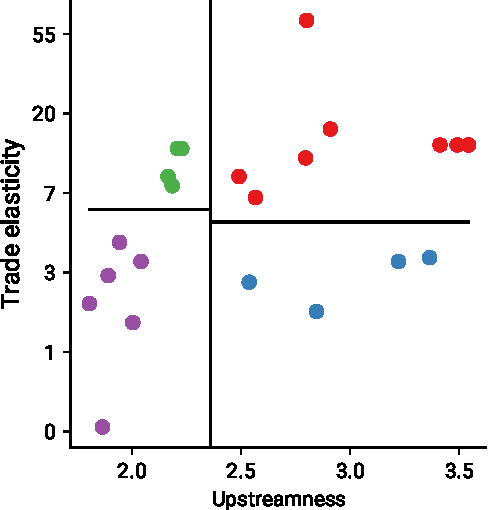
\includegraphics[width=\textwidth]{../programs/python/output/fig_data_upstream_vs_elast.pdf}
\end{figure}
    \end{column}
    


\begin{column}{0.59\textwidth}    
\begin{table}
\renewcommand{\arraystretch}{1.75}
\begin{center}
\caption*{Sectoral aggregation}
\resizebox{\textwidth}{!}{%
\begin{tabular}{lp{6cm}cccc}\toprule
Sector & Industries & Upstreamness & \makecell{Trade\\elasticity} & \makecell{Share of\\mfg. emp.}\\
\midrule
\textcolor[HTML]{e41a1c}{``Oil''} & Agriculture, Mining (energy), Mining (non-energy), Mining support, Wood products, Paper products, Refined petroleum, Fabricated metals& 3.0& 17.6& 28.4\\
\textcolor[HTML]{377eb8}{``Steel''} & Chemicals, Rubber + plastics, Minerals, Basic metals& 3.0& 2.8& 18.1\\
\textcolor[HTML]{4daf4a}{``Toys''} & Fishing, Textiles, Electronics, Electrical equipment& 2.2& 11.9& 17.7\\
\textcolor[HTML]{984ea3}{``Cars''} & Food + beverages, Pharmateuticals, Machinery + equipment, Motor vehicles, Other trans. equip., Other mfg& 1.9& 2.2& 35.7\\
\bottomrule
\end{tabular}
}
\end{center}
\end{table}
    \end{column}

    \end{columns}

\end{frame}


%%%%%%%%%%%%%%%%%%%%%%%%%%%%%%%%%%%%%%%%%%%%%%%%%%%%%%%%%%%%%%%%%%%%%%%%%%%
\begin{frame}[noframenumbering,plain,t]{Supply-chain linkages}
\begin{figure}
\vspace{-0.35cm}
    \begin{subfigure}[t]{0.45\textwidth}
          \centering
         \caption*{Downstream: intermediate purchases (\% gross output)\\{\scriptsize{\textit{`If it gets more expensive, how much does it affect me?''}}}}
         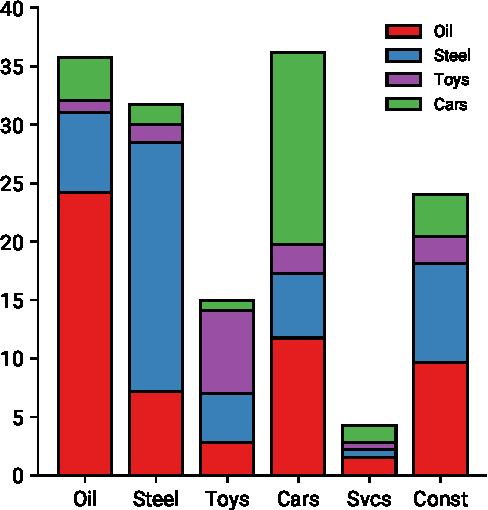
\includegraphics[width=\textwidth]{../programs/python/output/fig_data_linkages_downstream_0.pdf}
     \end{subfigure}
     \hfill
 \begin{subfigure}[t]{0.45\textwidth}
          \centering
         \caption*{Upstream: intermediate sales (\% gross output)\\{\scriptsize{\textit{``If they stop buying, how much does it affect me?''}}}}
         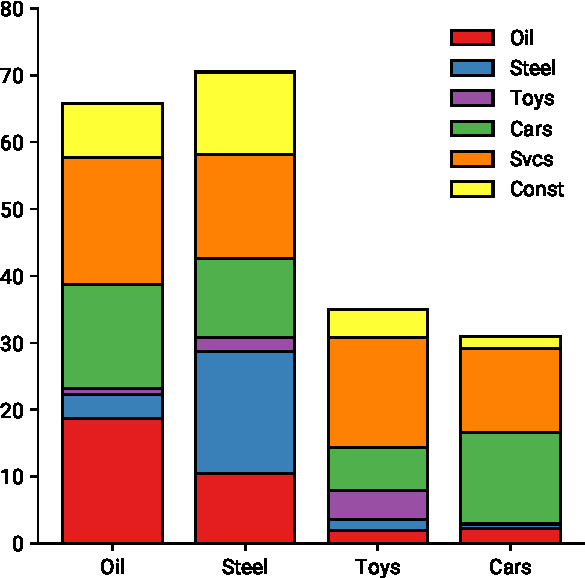
\includegraphics[width=\textwidth]{../programs/python/output/fig_data_linkages_upstream_0.pdf}
     \end{subfigure}
\end{figure}
\end{frame}


\begin{comment}
%%%%%%%%%%%%%%%%%%%%%%%%%%%%%%%%%%%%%%%%%%%%%%%%%%%%%%%%%%%%%%%%%%%%%%%%%%%
\begin{frame}[noframenumbering,plain,t]{Sectoral exposure to trade: by source country}
\begin{figure}
   %    \begin{subfigure}[t]{0.32\textwidth}
   %       \centering
   %      \caption*{Exports (\% sectoral value added)}
   %      \includegraphics[width=\textwidth]{../programs/python/output/fig_data_sectoral_trade_ex.pdf}
   %  \end{subfigure}
    \begin{subfigure}[t]{0.45\textwidth}
          \centering
         \caption*{Imports (\% sectoral gross output)}
         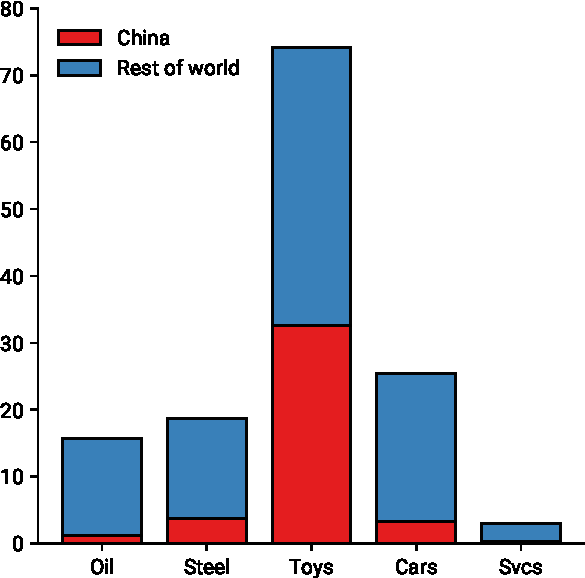
\includegraphics[width=\textwidth]{../programs/python/output/fig_data_sectoral_trade_by_region_im.pdf}
     \end{subfigure}
 \begin{subfigure}[t]{0.45\textwidth}
          \centering
         \caption*{Trade balance (\% sectoral gross output)}
         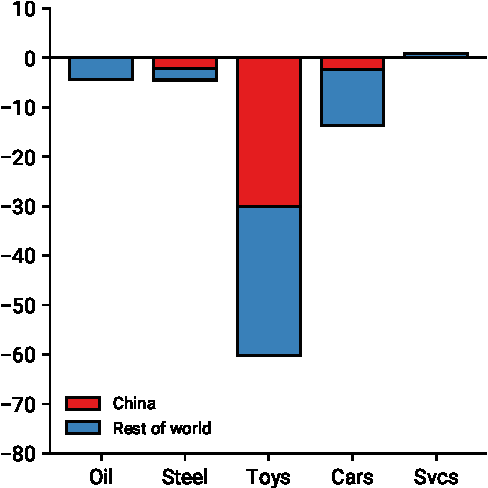
\includegraphics[width=\textwidth]{../programs/python/output/fig_data_sectoral_trade_by_region_nx.pdf}
     \end{subfigure}
\end{figure}
\end{frame}

%%%%%%%%%%%%%%%%%%%%%%%%%%%%%%%%%%%%%%%%%%%%%%%%%%%%%%%%%%%%%%%%%%%%%%%%%%%
\begin{frame}[noframenumbering,plain,t]{Macroeconomic importance of trade: by source country}
\begin{figure}
  %     \begin{subfigure}[t]{0.32\textwidth}
  %        \centering
  %       \caption*{Exports (\% GDP)}
  %       \includegraphics[width=\textwidth]{../programs/python/output/fig_data_sectoral_trade_ex2.pdf}
  %   \end{subfigure}
    \begin{subfigure}[t]{0.45\textwidth}
          \centering
         \caption*{Imports (\% GDP)}
         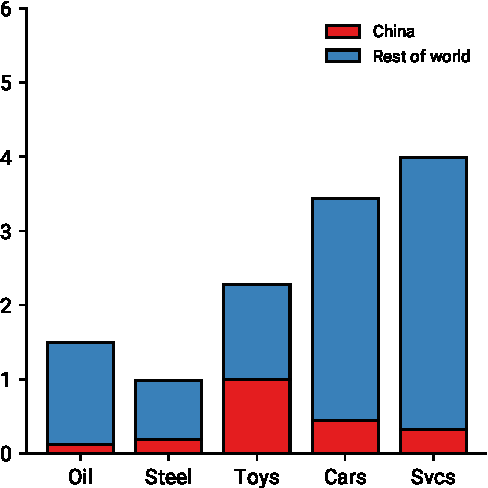
\includegraphics[width=\textwidth]{../programs/python/output/fig_data_sectoral_trade_by_region_im2.pdf}
     \end{subfigure}
 \begin{subfigure}[t]{0.45\textwidth}
          \centering
         \caption*{Trade balance (\% GDP)}
         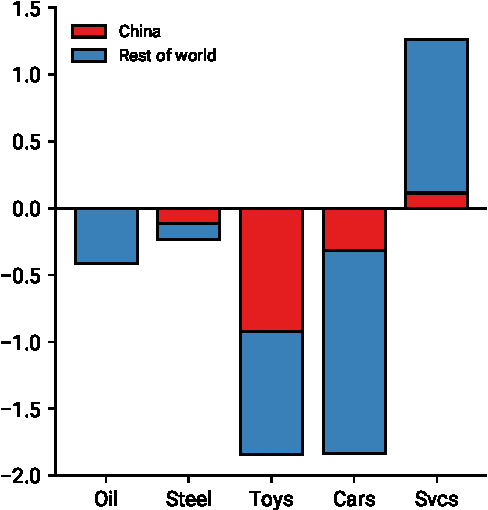
\includegraphics[width=\textwidth]{../programs/python/output/fig_data_sectoral_trade_by_region_nx2.pdf}
     \end{subfigure}
\end{figure}
\end{frame}
\end{comment}

%%%%%%%%%%%%%%%%%%%%%%%%%%%%%%%%%%%%%%%%%%%%%%%%%%%%%%%%%%%%%%%%%%%%%%%%%%%
\begin{frame}[noframenumbering,plain,t]{Sectoral exposure to trade}
\vspace{-0.35cm}
\begin{figure}
   %    \begin{subfigure}[t]{0.32\textwidth}
   %       \centering
   %      \caption*{Exports (\% sectoral value added)}
   %      \includegraphics[width=\textwidth]{../programs/python/output/fig_data_sectoral_trade_ex.pdf}
   %  \end{subfigure}
    \begin{subfigure}[t]{0.45\textwidth}
          \centering
         \caption*{Imports (\% sectoral gross output)}
         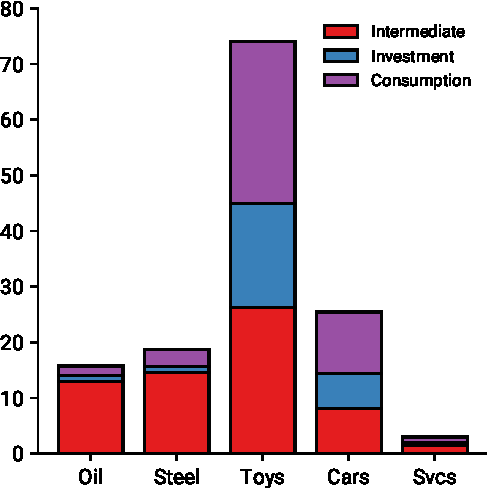
\includegraphics[width=\textwidth]{../programs/python/output/fig_data_sectoral_trade_by_use_im.pdf}
     \end{subfigure}
     \hfill
 \begin{subfigure}[t]{0.45\textwidth}
          \centering
         \caption*{Trade balance (\% sectoral gross output)}
         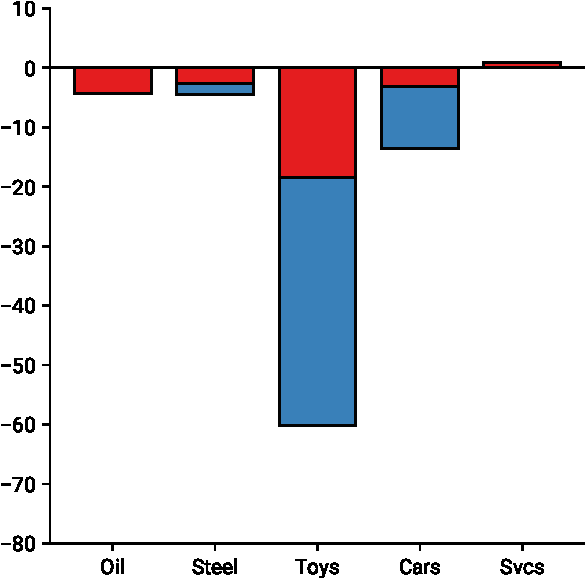
\includegraphics[width=\textwidth]{../programs/python/output/fig_data_sectoral_trade_by_use_nx.pdf}
     \end{subfigure}
\end{figure}
\end{frame}

%%%%%%%%%%%%%%%%%%%%%%%%%%%%%%%%%%%%%%%%%%%%%%%%%%%%%%%%%%%%%%%%%%%%%%%%%%%
\begin{frame}[noframenumbering,plain,t]{Macroeconomic importance of trade}
\vspace{-0.35cm}
\begin{figure}
  %     \begin{subfigure}[t]{0.32\textwidth}
  %        \centering
  %       \caption*{Exports (\% GDP)}
  %       \includegraphics[width=\textwidth]{../programs/python/output/fig_data_sectoral_trade_ex2.pdf}
  %   \end{subfigure}
    \begin{subfigure}[t]{0.45\textwidth}
          \centering
         \caption*{Imports (\% GDP)}
         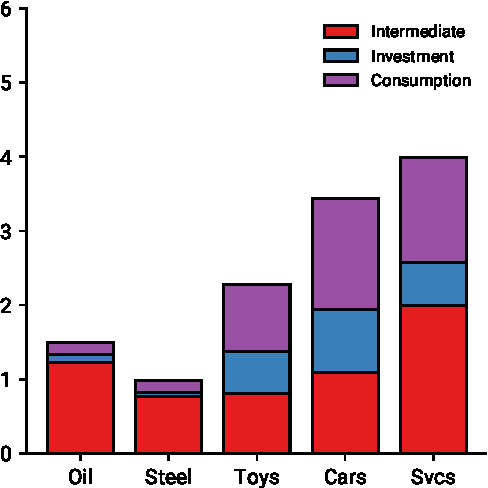
\includegraphics[width=\textwidth]{../programs/python/output/fig_data_sectoral_trade_by_use_im2.pdf}
     \end{subfigure}
     \hfill
 \begin{subfigure}[t]{0.45\textwidth}
          \centering
         \caption*{Trade balance (\% GDP)}
         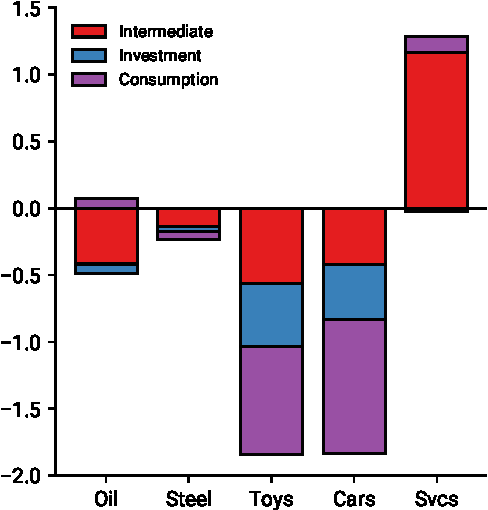
\includegraphics[width=\textwidth]{../programs/python/output/fig_data_sectoral_trade_by_use_nx2.pdf}
     \end{subfigure}
\end{figure}
\end{frame}

%%%%%%%%%%%%%%%%%%%%%%%%%%%
%%%%%%%%%%%%%%%%%%%%%%%%%%%
\begin{transitionframe}
Experiments
\end{transitionframe}

%%%%%%%%%%%%%%%%%%%%%%%%%
%%%%%%%%%%%%%%%%%%%%%%%%%
\begin{frame}[noframenumbering,plain,t]
  \frametitle{Overview}
  \begin{itemize}\addtolength{\itemsep}{1ex}
  \item Start from steady state with free trade
  \item 25\% tariffs unexpected and permanent
  \begin{itemize}
      \item On each good separately
      \item On all goods together
  \end{itemize}
  \item Object of interest: goods-sector employment dynamics
  \end{itemize}
\end{frame}

%%%%%%%%%%%%%%%%%%%%%%%%%%%%%%%%%%%%%%%%%%%%%%%%%%%%%%%%%%%%%%%%%%%%%%%%%%%
\begin{frame}[noframenumbering,plain,t]{Which tariffs would be most effective at reindustrialization?}

\begin{columns}

    \begin{column}{0.45\textwidth}
    \begin{figure}
    \centering
    %\caption*{Effect on total goods emp}
    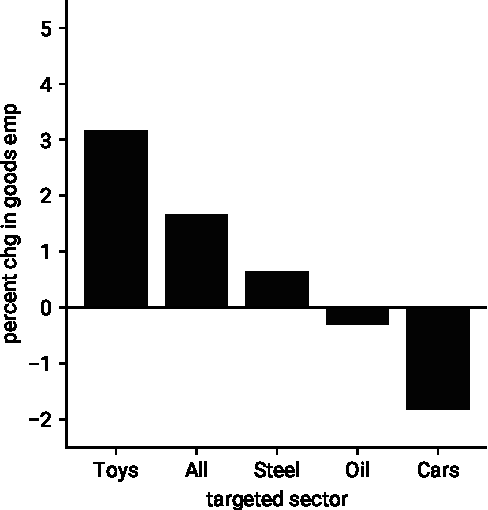
\includegraphics[width=\textwidth]{../programs/python/output/fig_lr_emp_across_scenarios_all.pdf}
\end{figure}
    \end{column}  
\hfill

\begin{column}{0.54\textwidth}    
\begin{itemize}
\addtolength{\itemsep}{1ex}
    \item Best: high-elasticity, downstream goods (``toys'')
    \item Worst: low-elasticity, downstream goods (``cars'')
    \item Broadest: Across-the-board (ATB) tariff on all goods. Still generates smaller employment gain than tariff on toys only.
\end{itemize}
    \end{column}
    \end{columns}

\end{frame}

%%%%%%%%%%%%%%%%%%%%%%%%%%%%%%%%%%%%%%%%%%%%%%%%%%%%%%%%%%%%%%%%%%%%%%%%%%%
\begin{frame}[noframenumbering,plain,t]{Reindustrialization or reallocation?}

\begin{columns}

    \begin{column}{0.45\textwidth}
    \begin{figure}
    \centering
    %\caption*{Effect on total goods emp}
    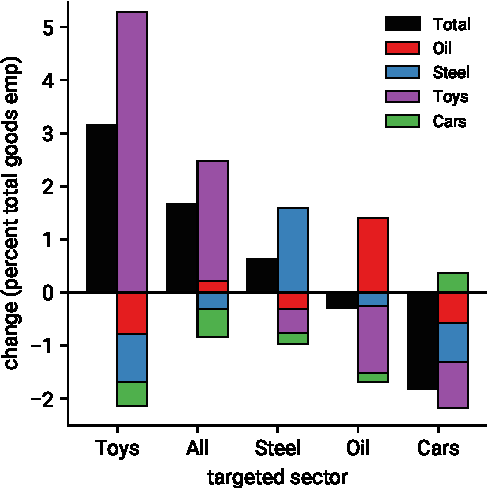
\includegraphics[width=\textwidth]{../programs/python/output/fig_lr_emp_across_scenarios_all_vs_sectors.pdf}
\end{figure}
    \end{column}  
\hfill

\begin{column}{0.54\textwidth}    
\begin{itemize}
\addtolength{\itemsep}{1ex}
    \item Employment gains concentrated in one sector. All other sectors lose workers.
    \item ATB tariff hurts low-elasticity sectors. Barely helps ``oil.'' Less growth in ``toys'' than under targeted tariff.
    \item Tariff on ``cars'' hurts all other sectors more than it helps protected sector
\end{itemize}
    \end{column}
    \end{columns}

\end{frame}


%%%%%%%%%%%%%%%%%%%%%%%%%%%%%%%%%%%%%%%%%%%%%%%%%%%%%%%%%%%%%%%%%%%%%%%%%%%
\begin{frame}[noframenumbering,plain,t]{Short run vs. long run}

\begin{columns}

    \begin{column}{0.45\textwidth}
    \vspace{-0.25cm}
    \begin{figure}
    \centering
    \only<1>{\caption*{Employment dynamics: ``toys'' only}}
    \only<2>{\caption*{Employment dynamics: all}}
    \only<3>{\caption*{Employment dynamics: ``steel'' only}}
    \only<4>{\caption*{Employment dynamics: ``oil'' only}}
    \only<5>{\caption*{Employment dynamics: ``cars'' only}}
    
    \only<1>{
    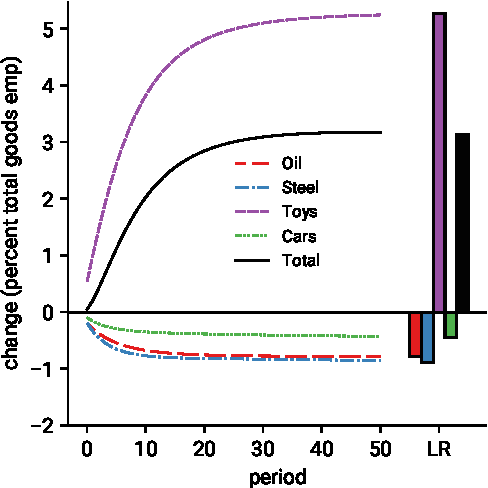
\includegraphics[width=\textwidth]{../programs/python/output/fig_dyn_labor_goods_s2.pdf}
    }

    \only<2>{
    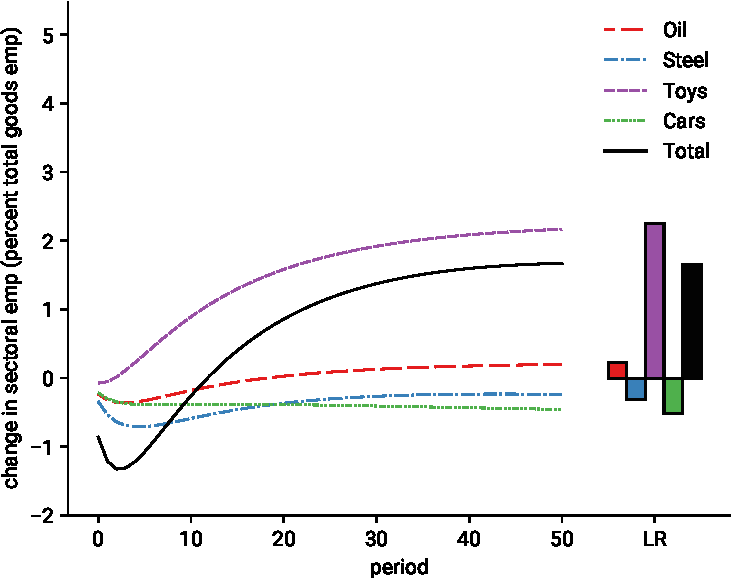
\includegraphics[width=\textwidth]{../programs/python/output/fig_dyn_labor_goods_s4.pdf}
    }

    \only<3>{
    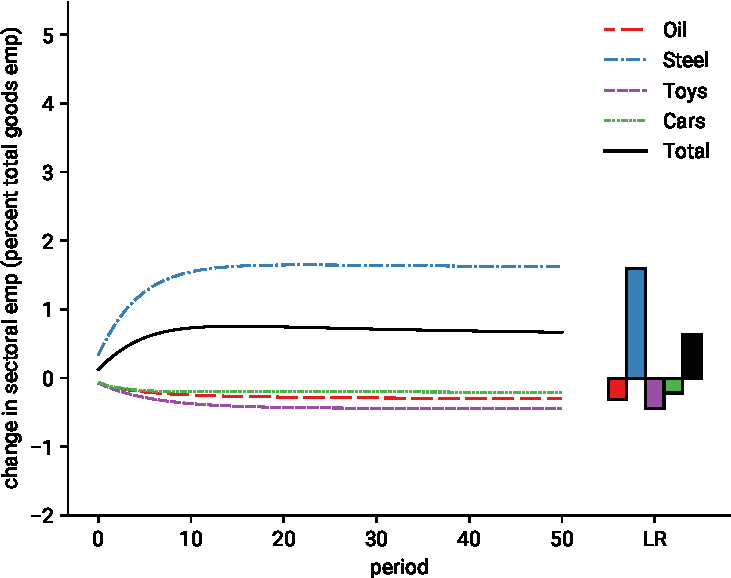
\includegraphics[width=\textwidth]{../programs/python/output/fig_dyn_labor_goods_s1.pdf}
    }

    \only<4>{
    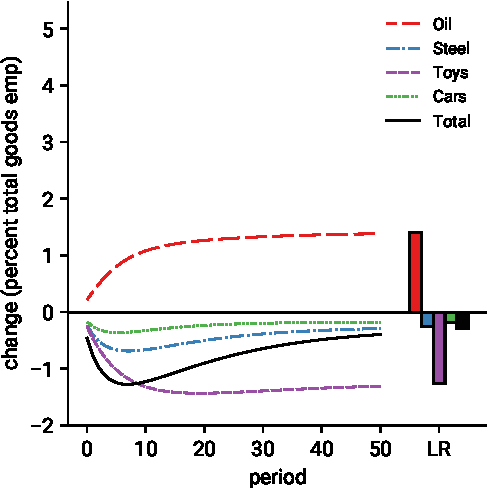
\includegraphics[width=\textwidth]{../programs/python/output/fig_dyn_labor_goods_s0.pdf}
    }

    \only<5>{
    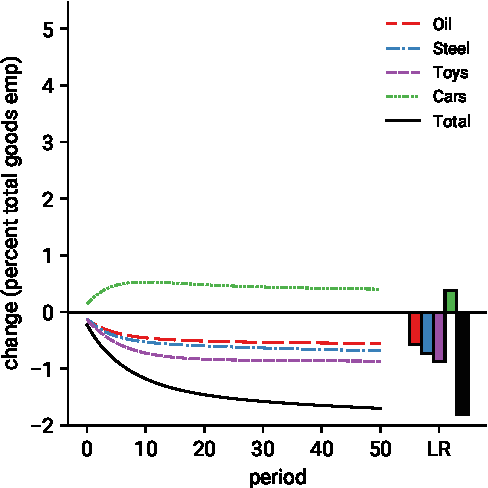
\includegraphics[width=\textwidth]{../programs/python/output/fig_dyn_labor_goods_s3.pdf}
    }
    
\end{figure}
    \end{column}  
\hfill

\begin{column}{0.54\textwidth}    
\begin{itemize}
\addtolength{\itemsep}{1ex}
    \item<1-> ``Toys:'' Gradual net growth \& reallocation
    \item<2-> All: Overall employment falls in SR. ``Toys'' grows gradually, other sectors overshoot.
    \item<3-> ``Steel:'' Gradual growth \& reallocation. Faster than ``toys'' tariff, but smaller effects.
    \item<4-> ``Oil:'' Pronounced overshooting in overall employment, steel \& cars
    \item<5-> ``Cars:'' Gradual net contraction \& reallocation
\end{itemize}
    \end{column}
    \end{columns}

\end{frame}



%%%%%%%%%%%%%%%%%%%%%%%%%
%%%%%%%%%%%%%%%%%%%%%%%%%
\begin{frame}[noframenumbering,plain,t]
  \frametitle{Other considerations}
  \begin{itemize}\addtolength{\itemsep}{1ex}
  \item What about macroeconomic consequences?
  \item Target all countries or just China?
    \item What if other countries retaliate?
    \item What if there were no adjustment frictions?
    %\item What if the tariffs end after Trump's term in office?
    \item For simplicity, focus on across-the-board tariffs on all goods sectors
    \end{itemize}
\end{frame}

%%%%%%%%%%%%%%%%%%%%%%%%%%%%%%%%%%%%%%%%%%%%%%%%%%%%%%%%%%%%%%%%%%%%%%%%%%%
\begin{frame}[noframenumbering,plain,t]{Goods employment vs. aggregate GDP}
    \vspace{-0.35cm}
\begin{columns}

    \begin{column}{0.45\textwidth}
    \begin{figure}
    \centering
    \caption*{Long-run effects}
    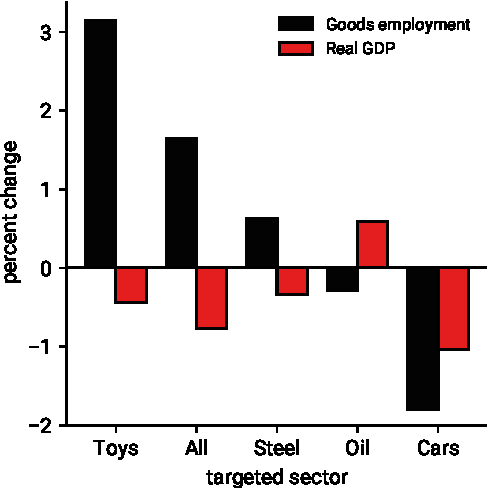
\includegraphics[width=\textwidth]{../programs/python/output/fig_lr_emp_vs_gdp.pdf}
\end{figure}
    \end{column}  
\hfill
    \begin{column}{0.45\textwidth}
    \begin{figure}
    \centering
    \caption*{GDP dynamics}
    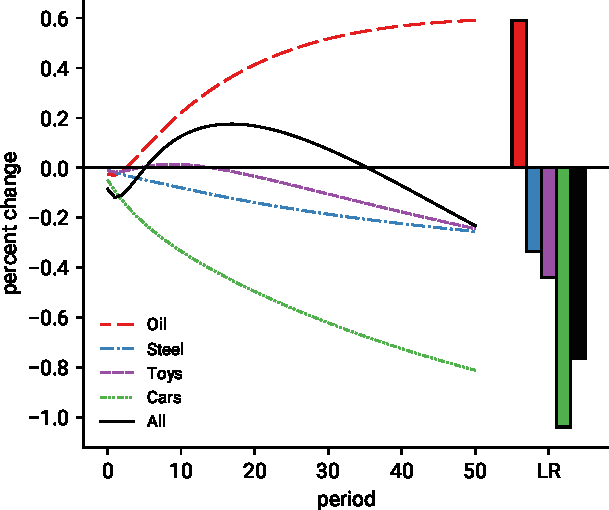
\includegraphics[width=\textwidth]{../programs/python/output/fig_dyn_macro.pdf}
\end{figure}
    \end{column}  

    \end{columns}

\end{frame}

%%%%%%%%%%%%%%%%%%%%%%%%%%%%%%%%%%%%%%%%%%%%%%%%%%%%%%%%%%%%%%%%%%%%%%%%%%%
\begin{frame}[noframenumbering,plain,t]{Target all countries or just China?}
    \vspace{-0.35cm}
\begin{columns}

    \begin{column}{0.45\textwidth}
    \begin{figure}
    \centering
    \caption*{Effect on total goods emp}
    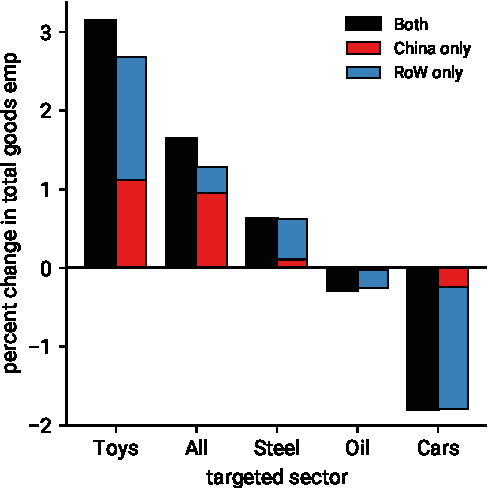
\includegraphics[width=\textwidth]{../programs/python/output/fig_lr_emp_across_scenarios_compare.pdf}
\end{figure}
    \end{column}  

\hfill
\begin{column}{0.54\textwidth}    
\begin{itemize}
\addtolength{\itemsep}{1ex}
    \item Targeting only one country diverts trade to the other, reducing domestic production boost
    \item Especially in high-elasticity sectors where substituting between import sources is easy
    \begin{itemize}
        \item Most diversion in ``toys'', least in ``cars'' \& ``steel''
    \end{itemize}
    \item Less diversion when one country is a minor supplier
    \begin{itemize}
        \item ``Oil'' has a high elasticity, but little potential for diversion because US buys barely any from China
    \end{itemize}
\end{itemize}
    \end{column}
    \end{columns}

\end{frame}

%%%%%%%%%%%%%%%%%%%%%%%%%%%%%%%%%%%%%%%%%%%%%%%%%%%%%%%%%%%%%%%%%%%%%%%%%%%
\begin{frame}[noframenumbering,plain,t]{Effects of retaliation}
    \vspace{-0.35cm}
\begin{columns}

    \begin{column}{0.45\textwidth}
    \begin{figure}
    \centering
    \caption*{Baseline model}
    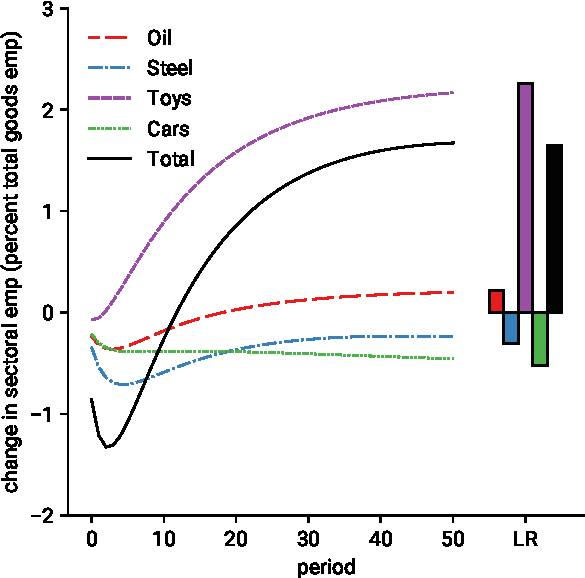
\includegraphics[width=\textwidth]{../programs/python/output/fig_dyn_labor_goods_atb_resize.pdf}
\end{figure}
    \end{column}
\hfill
\begin{column}{0.45\textwidth}    
 \begin{figure}
    \centering
    \caption*{With retaliation}
    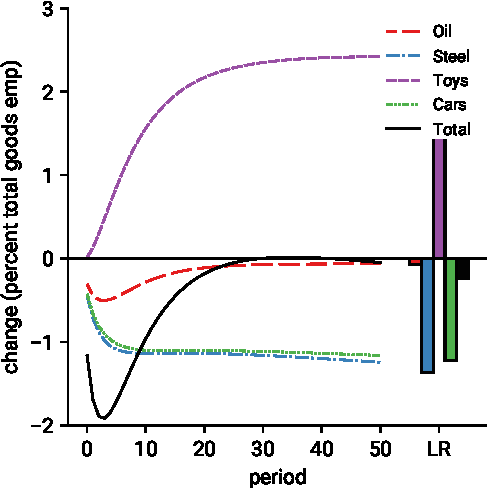
\includegraphics[width=\textwidth]{../programs/python/output/fig_dyn_labor_goods_atb_retaliation.pdf}
\end{figure}
    \end{column}
    \end{columns}

\end{frame}

%%%%%%%%%%%%%%%%%%%%%%%%%%%%%%%%%%%%%%%%%%%%%%%%%%%%%%%%%%%%%%%%%%%%%%%%%%%
\begin{frame}[noframenumbering,plain,t]{Effects of adjustment frictions}
  \vspace{-0.35cm}
\begin{columns}

    \begin{column}{0.45\textwidth}
    \begin{figure}
    \centering
    \caption*{Baseline model}
    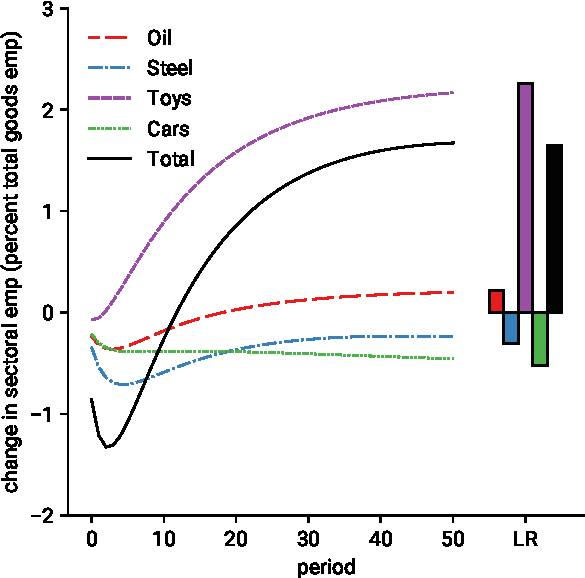
\includegraphics[width=\textwidth]{../programs/python/output/fig_dyn_labor_goods_atb_resize.pdf}
\end{figure}
    \end{column}
\hfill
\begin{column}{0.45\textwidth}    
 \begin{figure}
    \centering
    \caption*{Frictionless model}
    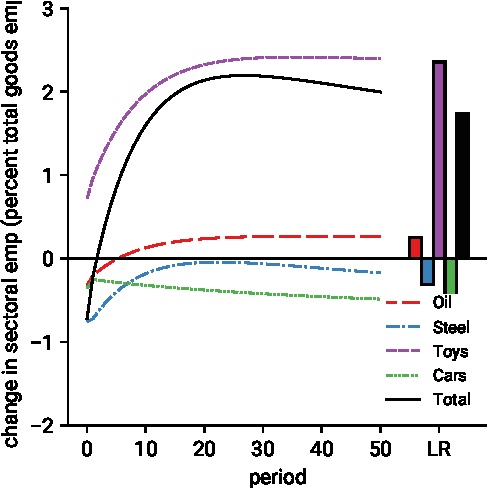
\includegraphics[width=\textwidth]{../programs/python/output/fig_dyn_labor_goods_atb_noadj.pdf}
\end{figure}
    \end{column}
    \end{columns}

\end{frame}

\begin{comment}
%%%%%%%%%%%%%%%%%%%%%%%%%%%%%%%%%%%%%%%%%%%%%%%%%%%%%%%%%%%%%%%%%%%%%%%%%%%
\begin{frame}[noframenumbering,plain,t]{Temporary vs. permanent}
  \vspace{-0.35cm}
\begin{columns}

    \begin{column}{0.45\textwidth}
    \begin{figure}
    \centering
    \caption*{Baseline model}
    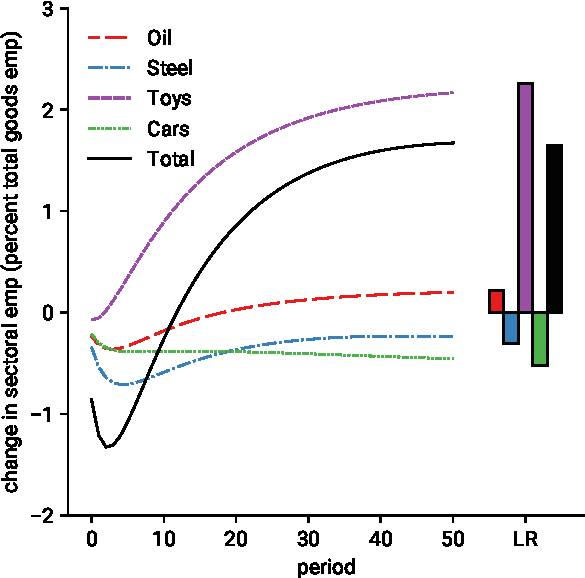
\includegraphics[width=\textwidth]{../programs/python/output/fig_dyn_labor_goods_atb_resize.pdf}
\end{figure}
    \end{column}
\hfill
\begin{column}{0.45\textwidth}    
 \begin{figure}
    \centering
    \caption*{Tariffs end unexpectedly after 4 years}
    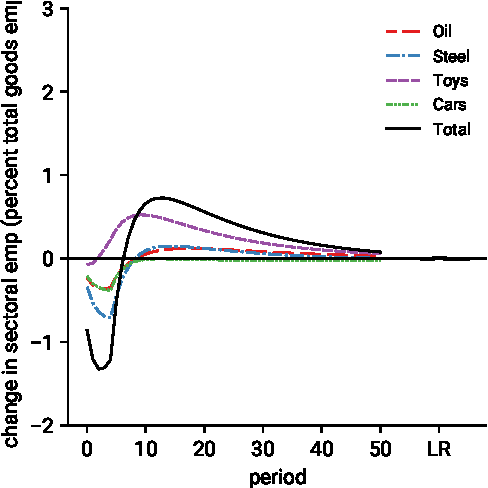
\includegraphics[width=\textwidth]{../programs/python/output/fig_dyn_labor_goods_atb_temp.pdf}
\end{figure}
    \end{column}
    \end{columns}

\end{frame}
\end{comment}

%%%%%%%%%%%%%%%%%%%%%%%%%%%
%%%%%%%%%%%%%%%%%%%%%%%%%%%
\begin{transitionframe}
Conclusion
\end{transitionframe}

%%%%%%%%%%%%%%%%%%%%%%%%%
%%%%%%%%%%%%%%%%%%%%%%%%%
\begin{frame}[noframenumbering,plain,t]
  \frametitle{Summary}
  \begin{itemize}\addtolength{\itemsep}{1ex}
  \item Can tariffs increase mfg employment? Yes, but with some caveats.
    \item Long-run gain may require short-term pain
    \begin{itemize}
    \item Employment can fall for 10+ years before rising
        \item Supply-chain adjustment frictions play crucial role. W/o frictions, employment rises immediately.
    \end{itemize}
      \item More reallocation across mfg industries than overall reindustrialization
      \begin{itemize}
      \item Broad tariffs only boost employment in consumer goods (``toys''). All other mfg industries shrink.
          \item Targeted tariffs can raise employment in industries with nat-sec concerns (cars, heavy machinery, etc.), but may shrink overall mfg sector
      \end{itemize}    
      \item Gains only possible if targeted countries don't retaliate
      \begin{itemize}
          \item With retaliation, no gain in long run and more pain in short run
      \end{itemize}
    \end{itemize}
\end{frame}


%%%%%%%%%%%%%%%%%%%%%%%%%
%%%%%%%%%%%%%%%%%%%%%%%%%
\begin{frame}[noframenumbering,plain,t]
  \frametitle{Parting thoughts}
  \begin{itemize}\addtolength{\itemsep}{1ex}
  \item Positive analysis only. Don't draw normative conclusions.
\item Manufacturing employment $!=$ welfare
\begin{itemize}
\item Welfare impact depends on what revenues are used for
    \item Consumption can rise in LR with lump-sum tariffs even though output falls
    \item But transition also matters! Next paper: optimal tariffs w/ vs. w/o supply-chain frictions.
\end{itemize}
      \item Hard to model and quantify nat-sec concerns
      \begin{itemize}
          \item Maybe gov't is willing to boost ``cars'' even if rest of mfg sector shrinks
      \end{itemize}
      \item $TFP = F(\text{tariffs})$?
      \begin{itemize}
          \item Protectionism often justified by scale/learning externality. But Baumol effect would attenuate effect on employment in equilibrium (Kehoe et al. 2018).
          \item But trade may also raise productivity (Atkeson-Burstein 2010). Could go other way!
      \end{itemize}
    \end{itemize}
\end{frame}

\appendix

%%%%%%%%%%%%%%%%%%%%%%%%%%%
%%%%%%%%%%%%%%%%%%%%%%%%%%%
\begin{transitionframe}
Appendix
\end{transitionframe}






%%%%%%%%%%%%%%%%%%%%%%%%%%%%%%%%%%%%%%%%%%%%%%%%%%%%%%%%%%%%%%%%%%%%%%%%%%%
\begin{frame}[noframenumbering,plain,t]{Gross output (pct changes)}
  \vspace{-0.6cm}

    \begin{figure}
    \centering
    \begin{subfigure}[t]{0.32\textwidth}
         \caption*{``Toys'' only}
         \vspace{-0.15cm}
    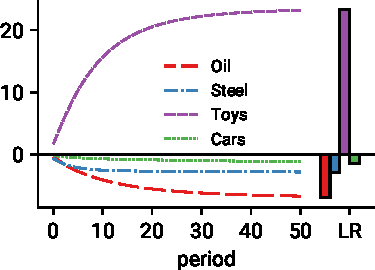
\includegraphics[width=\textwidth]{../programs/python/output/fig_dyn_y_goods_s2.pdf}
    \end{subfigure}
      \begin{subfigure}[t]{0.32\textwidth}
         \caption*{All goods}
         \vspace{-0.15cm}
    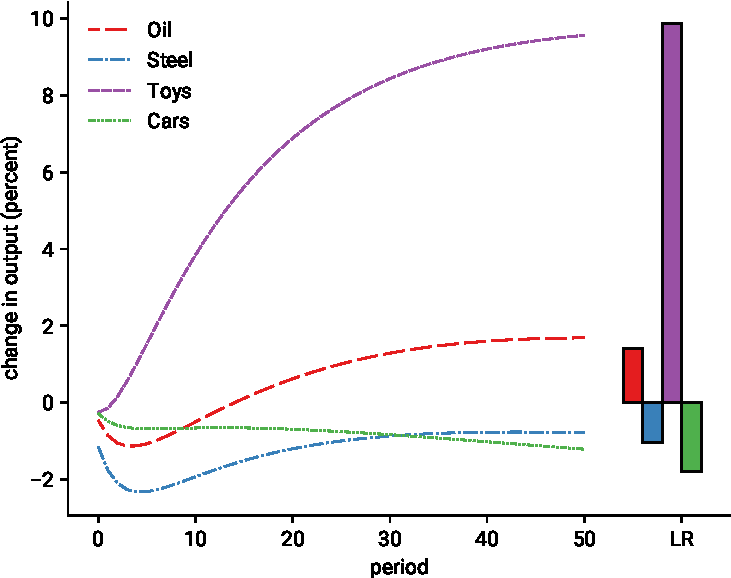
\includegraphics[width=\textwidth]{../programs/python/output/fig_dyn_y_goods_s4.pdf}
    \end{subfigure}
  \begin{subfigure}[t]{0.32\textwidth}
         \caption*{``Steel'' only}
         \vspace{-0.15cm}
    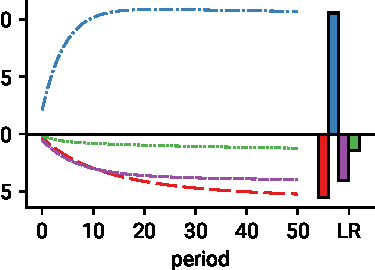
\includegraphics[width=\textwidth]{../programs/python/output/fig_dyn_y_goods_s1.pdf}
    \end{subfigure}
      \begin{subfigure}[t]{0.32\textwidth}
         \caption*{``Oil'' only''}
         \vspace{-0.15cm}
    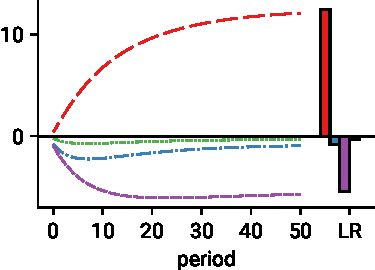
\includegraphics[width=\textwidth]{../programs/python/output/fig_dyn_y_goods_s0.pdf}
    \end{subfigure}   
      \begin{subfigure}[t]{0.32\textwidth}
         \caption*{``Cars'' only}
         \vspace{-0.15cm}
    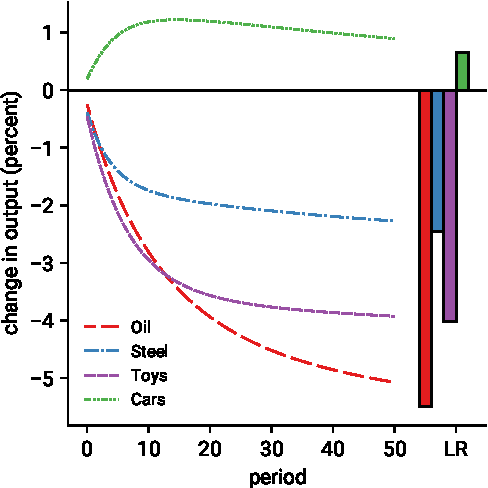
\includegraphics[width=\textwidth]{../programs/python/output/fig_dyn_y_goods_s3.pdf}
    \end{subfigure}  
\end{figure}

\end{frame}

%%%%%%%%%%%%%%%%%%%%%%%%%%%%%%%%%%%%%%%%%%%%%%%%%%%%%%%%%%%%%%%%%%%%%%%%%%%
\begin{frame}[noframenumbering,plain,t]{Imports (pct changes)}
  \vspace{-0.6cm}

    \begin{figure}
    \centering
    \begin{subfigure}[t]{0.32\textwidth}
         \caption*{``Toys'' only}
         \vspace{-0.15cm}
    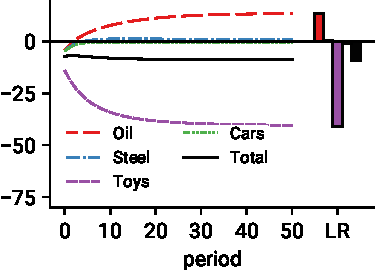
\includegraphics[width=\textwidth]{../programs/python/output/fig_dyn_imports_goods_s2.pdf}
    \end{subfigure}
      \begin{subfigure}[t]{0.32\textwidth}
         \caption*{All goods}
         \vspace{-0.15cm}
    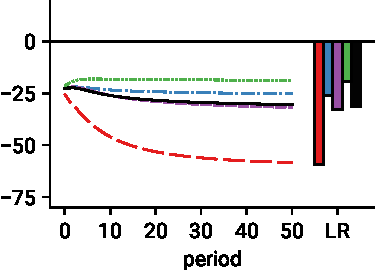
\includegraphics[width=\textwidth]{../programs/python/output/fig_dyn_imports_goods_s4.pdf}
    \end{subfigure}
  \begin{subfigure}[t]{0.32\textwidth}
         \caption*{``Steel'' only}
         \vspace{-0.15cm}
    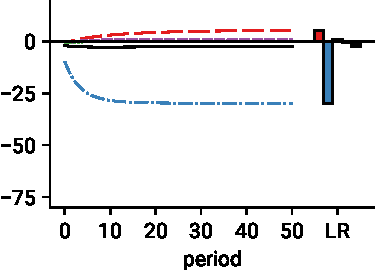
\includegraphics[width=\textwidth]{../programs/python/output/fig_dyn_imports_goods_s1.pdf}
    \end{subfigure}
      \begin{subfigure}[t]{0.32\textwidth}
         \caption*{``Oil'' only''}
         \vspace{-0.15cm}
    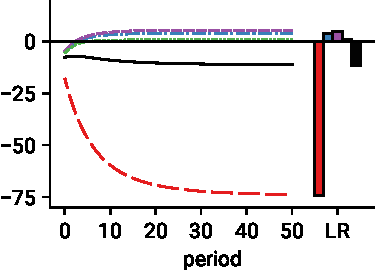
\includegraphics[width=\textwidth]{../programs/python/output/fig_dyn_imports_goods_s0.pdf}
    \end{subfigure}   
      \begin{subfigure}[t]{0.32\textwidth}
         \caption*{``Cars'' only}
         \vspace{-0.15cm}
    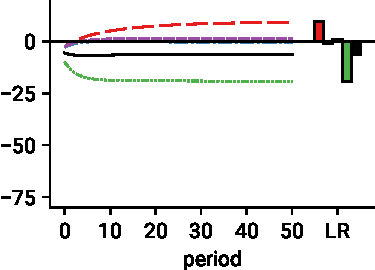
\includegraphics[width=\textwidth]{../programs/python/output/fig_dyn_imports_goods_s3.pdf}
    \end{subfigure}  
\end{figure}

\end{frame}

%%%%%%%%%%%%%%%%%%%%%%%%%%%%%%%%%%%%%%%%%%%%%%%%%%%%%%%%%%%%%%%%%%%%%%%%%%%
\begin{frame}[noframenumbering,plain,t]{Exports (pct changes)}
  \vspace{-0.6cm}

    \begin{figure}
    \centering
    \begin{subfigure}[t]{0.32\textwidth}
         \caption*{``Toys'' only}
         \vspace{-0.15cm}
    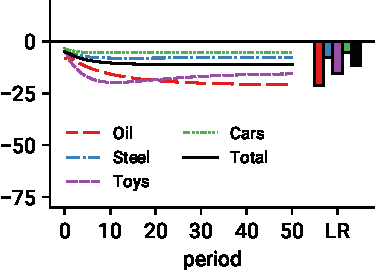
\includegraphics[width=\textwidth]{../programs/python/output/fig_dyn_exports_goods_s2.pdf}
    \end{subfigure}
      \begin{subfigure}[t]{0.32\textwidth}
         \caption*{All goods}
         \vspace{-0.15cm}
    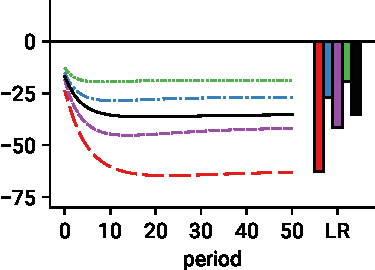
\includegraphics[width=\textwidth]{../programs/python/output/fig_dyn_exports_goods_s4.pdf}
    \end{subfigure}
  \begin{subfigure}[t]{0.32\textwidth}
         \caption*{``Steel'' only}
         \vspace{-0.15cm}
    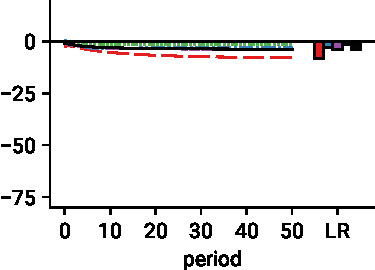
\includegraphics[width=\textwidth]{../programs/python/output/fig_dyn_exports_goods_s1.pdf}
    \end{subfigure}
      \begin{subfigure}[t]{0.32\textwidth}
         \caption*{``Oil'' only''}
         \vspace{-0.15cm}
    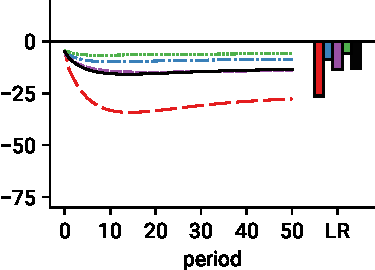
\includegraphics[width=\textwidth]{../programs/python/output/fig_dyn_exports_goods_s0.pdf}
    \end{subfigure}   
      \begin{subfigure}[t]{0.32\textwidth}
         \caption*{``Cars'' only}
         \vspace{-0.15cm}
    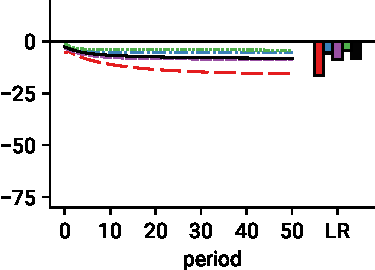
\includegraphics[width=\textwidth]{../programs/python/output/fig_dyn_exports_goods_s3.pdf}
    \end{subfigure}  
\end{figure}

\end{frame}

%%%%%%%%%%%%%%%%%%%%%%%%%%%%%%%%%%%%%%%%%%%%%%%%%%%%%%%%%%%%%%%%%%%%%%%%%%%
\begin{frame}[noframenumbering,plain,t]{Net exports/GDP (pp changes)}
  \vspace{-0.6cm}

    \begin{figure}
    \centering
    \begin{subfigure}[t]{0.32\textwidth}
         \caption*{``Toys'' only}
         \vspace{-0.15cm}
    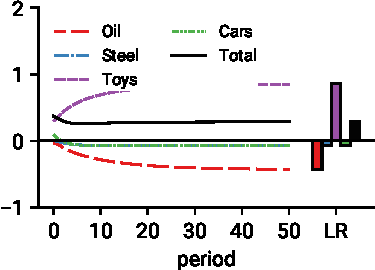
\includegraphics[width=\textwidth]{../programs/python/output/fig_dyn_nx_goods_s2.pdf}
    \end{subfigure}
      \begin{subfigure}[t]{0.32\textwidth}
         \caption*{All goods}
         \vspace{-0.15cm}
    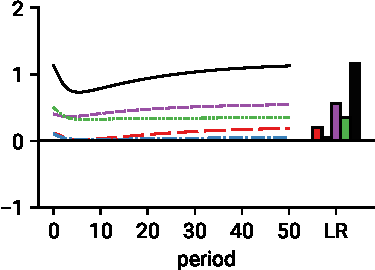
\includegraphics[width=\textwidth]{../programs/python/output/fig_dyn_nx_goods_s4.pdf}
    \end{subfigure}
  \begin{subfigure}[t]{0.32\textwidth}
         \caption*{``Steel'' only}
         \vspace{-0.15cm}
    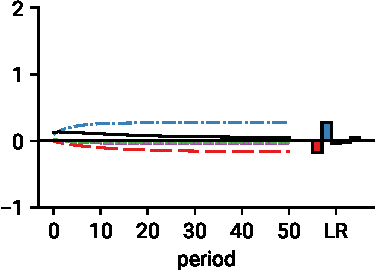
\includegraphics[width=\textwidth]{../programs/python/output/fig_dyn_nx_goods_s1.pdf}
    \end{subfigure}
      \begin{subfigure}[t]{0.32\textwidth}
         \caption*{``Oil'' only''}
         \vspace{-0.15cm}
    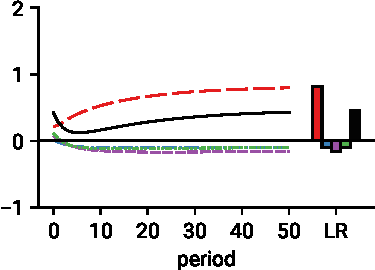
\includegraphics[width=\textwidth]{../programs/python/output/fig_dyn_nx_goods_s0.pdf}
    \end{subfigure}   
      \begin{subfigure}[t]{0.32\textwidth}
         \caption*{``Cars'' only}
         \vspace{-0.15cm}
    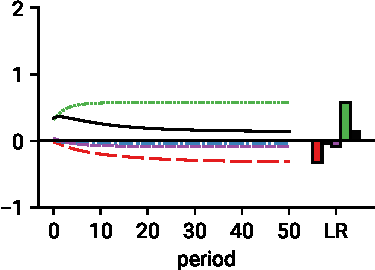
\includegraphics[width=\textwidth]{../programs/python/output/fig_dyn_nx_goods_s3.pdf}
    \end{subfigure}  
\end{figure}

\end{frame}

%%%%%%%%%%%%%%%%%%%%%%%%%%%%%%%%%%%%%%%%%%%%%%%%%%%%%%%%%%%%%%%%%%%%%%%%%%%
\begin{frame}[noframenumbering,plain,t]{Sector-level employment (pct changes)}
  \vspace{-0.6cm}

    \begin{figure}
    \centering
    \begin{subfigure}[t]{0.32\textwidth}
         \caption*{``Toys'' only}
         \vspace{-0.15cm}
    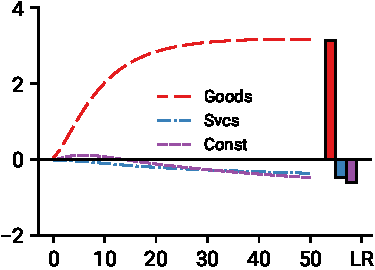
\includegraphics[width=\textwidth]{../programs/python/output/fig_dyn_labor_sectors_s2.pdf}
    \end{subfigure}
      \begin{subfigure}[t]{0.32\textwidth}
         \caption*{All goods}
         \vspace{-0.15cm}
    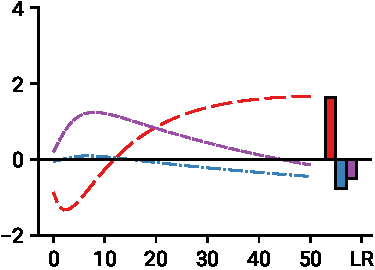
\includegraphics[width=\textwidth]{../programs/python/output/fig_dyn_labor_sectors_s4.pdf}
    \end{subfigure}
  \begin{subfigure}[t]{0.32\textwidth}
         \caption*{``Steel'' only}
         \vspace{-0.15cm}
    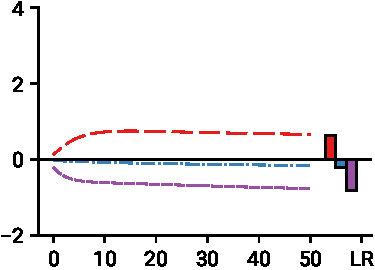
\includegraphics[width=\textwidth]{../programs/python/output/fig_dyn_labor_sectors_s1.pdf}
    \end{subfigure}
      \begin{subfigure}[t]{0.32\textwidth}
         \caption*{``Oil'' only''}
         \vspace{-0.15cm}
    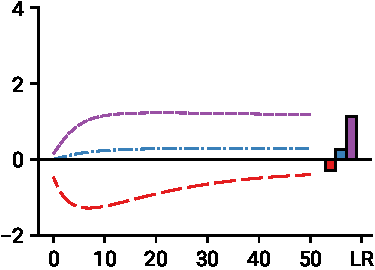
\includegraphics[width=\textwidth]{../programs/python/output/fig_dyn_labor_sectors_s0.pdf}
    \end{subfigure}   
      \begin{subfigure}[t]{0.32\textwidth}
         \caption*{``Cars'' only}
         \vspace{-0.15cm}
    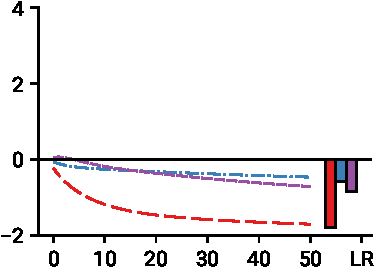
\includegraphics[width=\textwidth]{../programs/python/output/fig_dyn_labor_sectors_s3.pdf}
    \end{subfigure}  
\end{figure}
  

\end{frame}


%%%%%%%%%%%%%%%%%%%%%%%%%%%%%%%%%%%%%%%%%%%%%%%%%%%%%%%%%%%%%%%%%%%%%%%%%%%
\begin{frame}[noframenumbering,plain,t]{Intermediate goods prices (pct changes)}
  \vspace{-0.6cm}

    \begin{figure}
    \centering
    \begin{subfigure}[t]{0.32\textwidth}
         \caption*{``Toys'' only}
         \vspace{-0.15cm}
    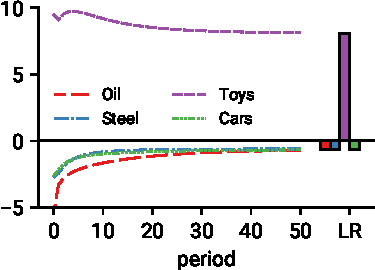
\includegraphics[width=\textwidth]{../programs/python/output/fig_dyn_pm_goods_s2.pdf}
    \end{subfigure}
      \begin{subfigure}[t]{0.32\textwidth}
         \caption*{All goods}
         \vspace{-0.15cm}
    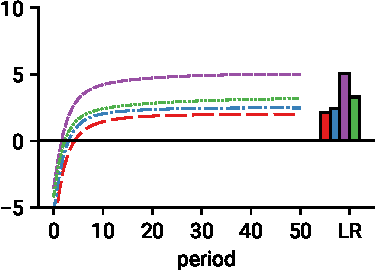
\includegraphics[width=\textwidth]{../programs/python/output/fig_dyn_pm_goods_s4.pdf}
    \end{subfigure}
  \begin{subfigure}[t]{0.32\textwidth}
         \caption*{``Steel'' only}
         \vspace{-0.15cm}
    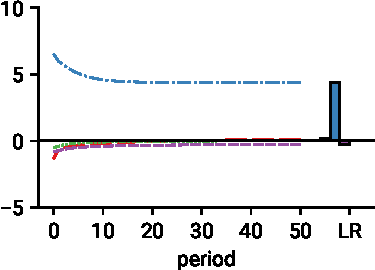
\includegraphics[width=\textwidth]{../programs/python/output/fig_dyn_pm_goods_s1.pdf}
    \end{subfigure}
      \begin{subfigure}[t]{0.32\textwidth}
         \caption*{``Oil'' only''}
         \vspace{-0.15cm}
    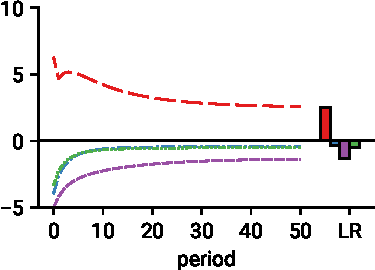
\includegraphics[width=\textwidth]{../programs/python/output/fig_dyn_pm_goods_s0.pdf}
    \end{subfigure}   
      \begin{subfigure}[t]{0.32\textwidth}
         \caption*{``Cars'' only}
         \vspace{-0.15cm}
    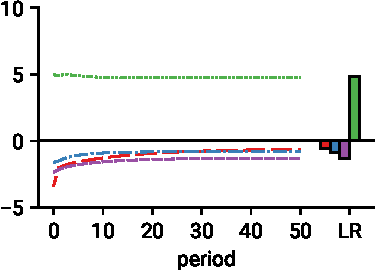
\includegraphics[width=\textwidth]{../programs/python/output/fig_dyn_pm_goods_s3.pdf}
    \end{subfigure}  
\end{figure}

\end{frame}

%%%%%%%%%%%%%%%%%%%%%%%%%%%%%%%%%%%%%%%%%%%%%%%%%%%%%%%%%%%%%%%%%%%%%%%%%%%
\begin{frame}[noframenumbering,plain,t]{Final goods prices (pct changes)}
  \vspace{-0.6cm}

    \begin{figure}
    \centering
    \begin{subfigure}[t]{0.32\textwidth}
         \caption*{``Toys'' only}
         \vspace{-0.15cm}
    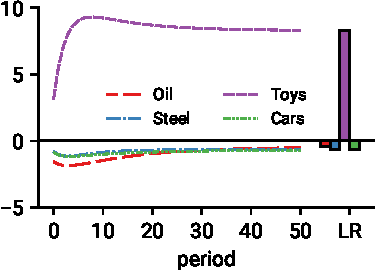
\includegraphics[width=\textwidth]{../programs/python/output/fig_dyn_pf_goods_s2.pdf}
    \end{subfigure}
      \begin{subfigure}[t]{0.32\textwidth}
         \caption*{All goods}
         \vspace{-0.15cm}
    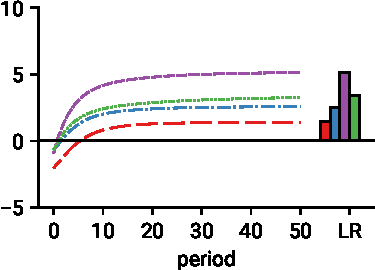
\includegraphics[width=\textwidth]{../programs/python/output/fig_dyn_pf_goods_s4.pdf}
    \end{subfigure}
  \begin{subfigure}[t]{0.32\textwidth}
         \caption*{``Steel'' only}
         \vspace{-0.15cm}
    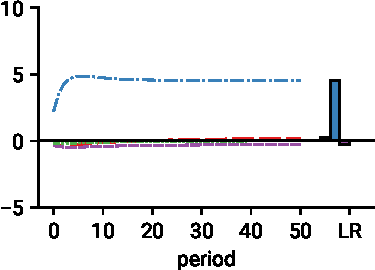
\includegraphics[width=\textwidth]{../programs/python/output/fig_dyn_pf_goods_s1.pdf}
    \end{subfigure}
      \begin{subfigure}[t]{0.32\textwidth}
         \caption*{``Oil'' only''}
         \vspace{-0.15cm}
    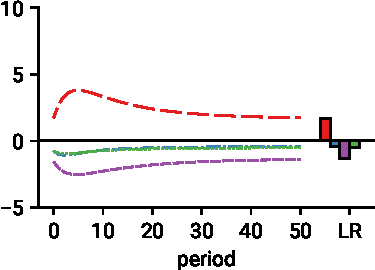
\includegraphics[width=\textwidth]{../programs/python/output/fig_dyn_pf_goods_s0.pdf}
    \end{subfigure}   
      \begin{subfigure}[t]{0.32\textwidth}
         \caption*{``Cars'' only}
         \vspace{-0.15cm}
    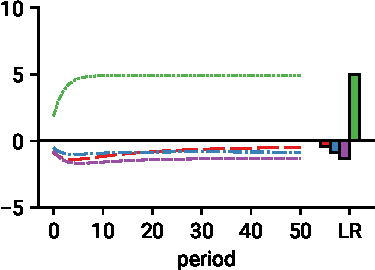
\includegraphics[width=\textwidth]{../programs/python/output/fig_dyn_pf_goods_s3.pdf}
    \end{subfigure}  
\end{figure}

\end{frame}






%%%%%%%%%%%%%%%%%%%%%%%%%%%%%%%%%%%%%%%%%%%%%%%%%%%%%%%%%%%%%%%%%%%%%%%%%%%
\end{document}
